\chapter{The CMS detector at the LHC}
\label{label: chapDetector}



The Large Hadron Collider (LHC) is the world$'$s largest and most powerful particle accelerator. 
Inside the accelerator, two high-energy particle beams travel at close to the speed of light before they are made to collide. The beams travel in opposite directions in separate beam pipes $-$two tubes kept at ultrahigh vacuum. They are guided around the accelerator ring by a strong magnetic field maintained by superconducting electromagnets.
The beams inside the LHC are made to collide at four locations around the accelerator ring, corresponding to the positions of four particle detectors � ATLAS, CMS, ALICE and LHCb.

%The prime motivation of the Large Hadron Collider (LHC) is to explore physics beyond the SM.  The Higgs discovery of the LHC is a tremendous success of experimental particle physics. The experimental study of the Higgs mechanism could shed light on the consistency of the SM and even drive to new physics. 
The focus of this chapter is to present a brief overview of the Compact Muon Solenoid (CMS) detector. 
The overall layout of CMS from different {\color{red}aspects} are shown in Figure~\ref{fig:CMSLayout} and Figure~\ref{fig:CMS_Slice}.   The dimensions of the CMS detectors are a length of 21.6 m, a diameter of 14.6 m and a total weight of 12500 tons.  In the following, we will first introduce the coordinates and then we will introduce the components of the CMS detector. 
%from the center,  along the diameter,  to the edge.
 
{\color{red} How to define the angles,
  $\eta \phi $
  Guofan's thesis has a good explanation of the angles. GOOD!
   What kind of information do I want to show in the 
detector section. A detailed one or a brief one, how brief. }




\begin{figure}
\centering
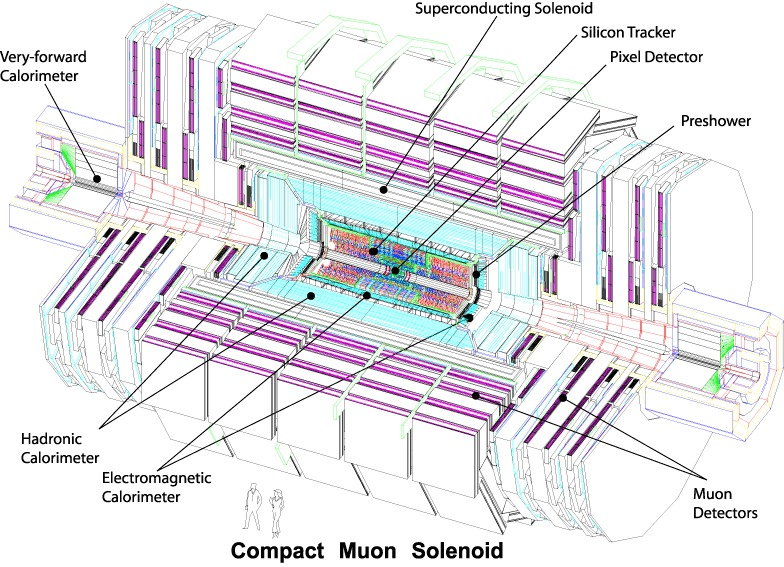
\includegraphics[width=.7\textwidth]{figures/cms_complete_layout.jpg}
\caption{An exploded view of the CMS detector.}
\label{figs:CMSLayout}
\end{figure}


\begin{figure}
\centering
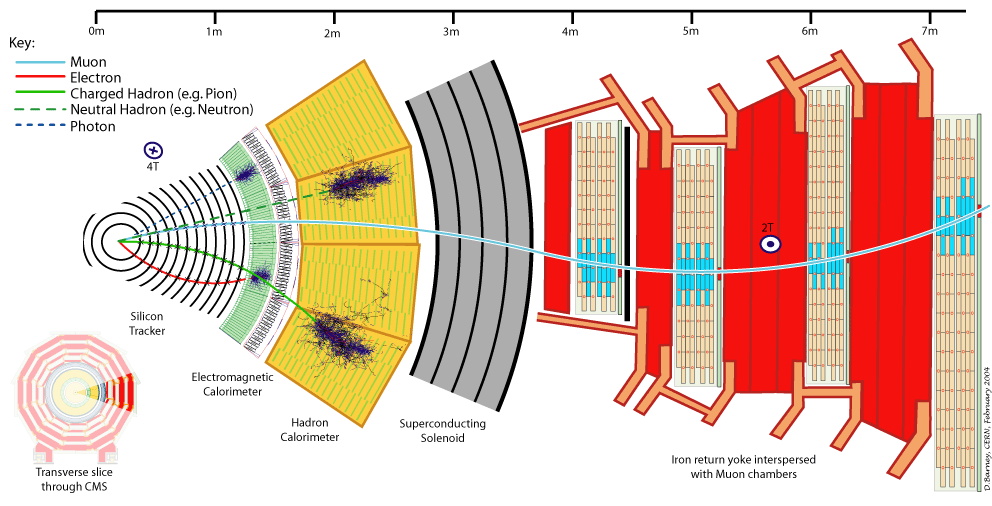
\includegraphics[width=.9\textwidth]{figures/CMS_Slice.png}
\caption{Transverse picture of the CMS detector. {\color{red} Change the picture to pdf format}}
\label{figs:CMS_Slice}
\end{figure}

\section{The beam: luminosity and cross-section}


\section{The coordinates}

\section{The Magnet}


In order to achieve good momentum resolution within a compact spectrometer without making stringent demands on muon-chamber resolution and alignment, a high magnetic field was chosen. The detailed parameters of this are shown in Table~\ref{table:magnet}.   The bore of the magnet coil is also large enough to accommodate the inner tracker and the calorimetry inside. 

\begin{table}[htb]
\caption{Parameters of the CMS superconducting solenoid.}
\begin{center}
\begin{tabular}{ |cc| }
\hline
Field           &  4 T \\
Inner Bore  &  5.9 m \\
Length        &  12.9 m \\
Number of turns &  2168 \\
Current   &        19.5 kA  \\
Store energy &  2.7 GJ \\
Hoop stress   &   64 atm \\
\hline
\end{tabular} 
\end{center}
\label{table:magnet}
\end{table}

\section{The inner tracking system}

{\color{red} Here we need a plot of the tracker layout and also the pixel tracker. If we could find a good description of the strip detector. }

The tracking volume is give by a cylinder of length 5.8 m and diameter 2.6 m.  In oder to deal with high track multiplicities, CMS employs 10 layers of silicon microstrip detectors, which provide the required granularity and precision.  In addition, 3 layers of silicon pixel detectors are placed closed to the interaction region to improve the measurement of impact parameter of charged-particle tracks, as well as the position of secondary vertices. 
The detailed layout of the tracker system is shown in Figure~\ref{fig:trackerLayout}

Close to the interaction vertex, in the barrel region, are 3 layers hybrid pixel detectors at a radii of 4.4, 7.3 and 10.2 cm.  
Each layer is spilt into segments like tiny kitchen tiles, each a little silicon sensor, 100 $\mu m$ by 
150 $\mu m$, about two hairs widths. Knowing which pixels have been touched allows us to deduce the particle$'$s trajectory. And because the detector is made of 2D tiles, rather than strips, and has a number of layers, we can create a three-dimensional picture.
The spatial resolution is measured to be $\approx$ 10 $\mu m$ for the $r-\phi$ measurement and $\approx$ 20 $\mu m$ for the $z$ measurement. 
After the pixels and on their way out of the tracker, particles pass through ten layers of silicon strip detectors, reaching out to a radius of 130 cm. The tracker silicon strip detector consists of four inner barrel (TIB) layers assembled in shells with two inner endcaps (TID), each composed of three small discs. The outer barrel (TOB) consists of six concentric layers. Finally two endcaps (TEC) close off the tracker. Each has silicon modules designed differently for its place within the detector.

\begin{figure}
\centering
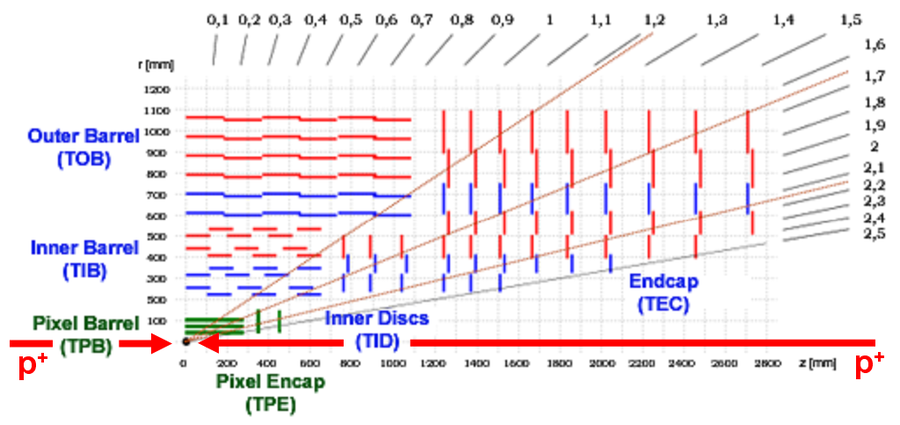
\includegraphics[width=1.4\textwidth]{figures/TrackerLayout.png}
\caption{The tracker layout of CMS}
\label{fig:trackerLayout}
\end{figure}

%In the barrel part, the silicon
%microstrip detectors are placed at $r$ between 20 and 110 cm.  The forward region has 2 pixel and 9 microstrip layers in each of the 2 endcaps.  The barrel part is separated into an Inner and an Outer Barrel.
%In order to avoid excessively shallow track crossing angles, the Inner Barrel is shorter than the Outer Barrel. 

% By considering the charged particle flux at various radii at high luminosity (Table~\ref{table:flux}), 3 regions can be delineated :
 
 %\begin{itemize}
 
 %\item  Closest to the interaction vertex where the particle flux is the highest ( $\approx 10^7 / s at r \approx 10 cm$), pixel detectors are placed, with an occupancy of about $10^{-4}$ per pixel per LHC crossing.  
 
 %\item In the intermediate region ( $20 < r < 55 cm$),  silicon microstrip detectors are used, leading to 
 %an occupancy of $\approx 2-3\% $/ LHC crossing. 
 
 %\item  In the outermost region ($r > 55 cm$) of the inner tracker, strip 
 
 %\end{itemize}  

\section{Electromagnetic calorimeter (ECAL) }

The ECAL is designed to calibrate the energy of electron and photons resulting from pp collisions, and its structure is shown in Figure~\ref{fig:ECAL} 
ECAL uses lead tungstate ($PbWO_4$) crystals with coverage in $|\eta|$ up to 3.0. 
This crystal is highly transparent and ``scintillates'' when electrons and photons pass through it, which  produces light in proportion to the particle$�$s energy. Although lead tungstate has short radiation (0.89 cm) and Moliere (2.2 cm) lengths, are also fast and radiation hard, it produces relatively low light yield. So the silicon avalanche photodiodes (APDs) are used as photodetectors in the ECAL barrel (EB) and 
 vacuum phototriodes (VPTs) in the ECAL endcap (EE). 
 
 
 \begin{figure}
\centering
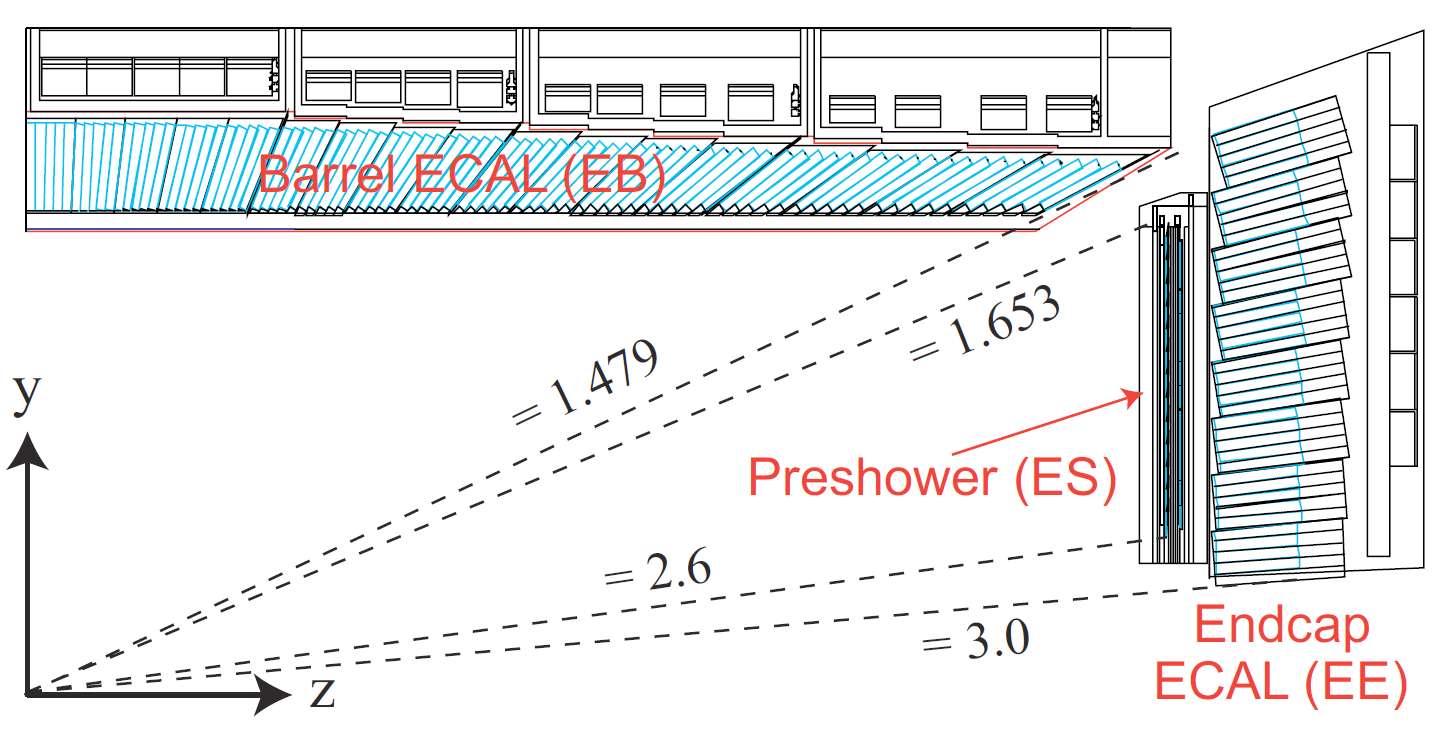
\includegraphics[width=.8\textwidth]{figures/ECALEta.png}
\caption{Geometric view of one quarter of the ECAL.}
\label{figs:ECAL}
\end{figure}

  
 These photodetectors that have been especially designed to work within the high magnetic field, are also glued onto the back of each of the crystals to detect the scintillation light and convert it to an electrical signal that is amplified and sent for analysis.
 
 A preshower system is installed in the front of EE.  
 The preshower is made of two planes of lead followed by silicon sensors, similar to those used in the tracker.  The reason for the preshower system is that short-lived particles called neutral pions, also produced in collisions, can inadvertently mimic high-energy photons when they decay into two closely-spaced lower energy photons that the ECAL picks up together. And for Higgs discovery,
 the high energy photons from Higgs decay is the important signature of $H \to \gamma \gamma$ channel. 
  

  \section{Hadronic calorimeter (HCAL)}
  
%  ECAL is surrounded by a brass/scintillator sampling hadron calorimeter with coverage up to $|\eta| < 3.0$. 



HCAL is designed to measure the energy of particles other than electron and photons, for example proton, neutron, pion and kaon.  It is also provide good containment and hermitically for the transverse missing energy $E_{T}^miss$ measurement, resulting from neutrinos or possible new particles. 

As shown in Figure~\ref{figs:HCAL},  HCAL is composed by four parts, HCAL barrel (HB), HCAL endocap (HE), HCAL outer (HO) and HCAL forward(HF).  HF is not presented in the plot. However, HF sits on the outside of the magnet and covers $3 <  |\eta| < 5.0$.  

HCAL is a brass/scintillator sampling hadron calorimeter. 
%{\bf HB}
 

\begin{figure}
\centering
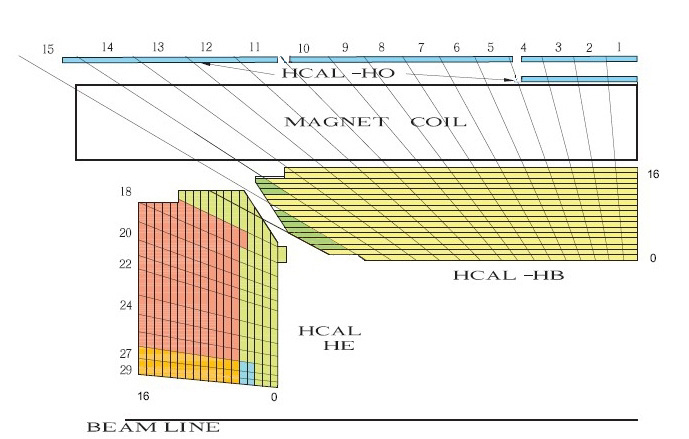
\includegraphics[width=.8\textwidth]{figures/Hcal.jpg}
\caption{Geometric view of one quarter of the HCAL. {\color{red} find a plot has HF}}
\label{figs:HCAL}
\end{figure}
  
  
\section{Muon system}
CMS is called the "compact muon solenoid". Muon detecting at CMS is very important. 
  
%Muons have a mass of 105.7 $MeV/c^2$, which is about 200 times that of the electron. Due to their greater mass, muons are not as sharply accelerated when they encounter electromagnetic fields, and do not emit as much bremsstrahlung (deceleration radiation). This allows muons of a given energy to penetrate far more deeply into matter than electrons, since the deceleration of electrons and muons is primarily due to energy loss by the bremsstrahlung mechanism. So muons could easily penetrate the ECAL. 
 
%Unlike hadron in HCAL, muon$'$s mass is much smaller than hadrons. Muon could 

Centrally produced muons are measured 3 times: in the inner tracker, after the coil , and in the return flux. Measurement of the momentum of muons using only the muon system is essentially determined by the muon bending angle at eh exit of the 4 T coil, taking the interaction point of pp collision as the origin of the muon.  For low-momentum muons, the best momentum resolution is given by the resolution 
obtained in the silicon tracker.  For high-momentum muons, combining the inner tracker and muon detector measurements will highly improve the muon momentum resolution.  
At CMS, in $0 < |\eta| < 2.0 $, for $\mu$ with $\pt$ $200 ~ 400$ GeV ,  $\delta p / p$ is measured to be $\leq 3\%$.


The layout of the one quarter of the CMS muon system for the initial low luminosity running is shown in 
Figure~\ref{fig:Muonsystem} and the transverse view of the muon stations (MS) are shown in 
Figure~\ref{fig:MuonStation}.  In the Muon Barrel (MB) region, 4 stations of detectors are arranged in cylinders interleaved with the iron yoke.  

Three types of gaseous detectors are used to identify and measure muons.{\color{red}cite some paper}. 
Drift tube (DT) is used in the barrel region ( $|\eta| < 1.2$).  In this region, the residual magnetic field in the chambers is low and also muon rate is low, so drift tube works well.  The maximum drift length is 2.0 cm and the single point resolution is $\approx$ 200 $\mu m$. 
In the endcap region,  cathode strip chambers (CSC) are used because of the high residual magnetic field and also high muon rate.  In addition to this,  resistive plate chambers (RPC) are used in both the barrel and the endcap regions. RPC could provide a fast response with good time resolution but with a coarser position resolutions than DTs and CSCs.  So RPC could identify the correct bunch crossing. 

\section{Trigger and data acuisistion}

%At LHC, protons collides 40 million times per second . 









\begin{figure}
\centering
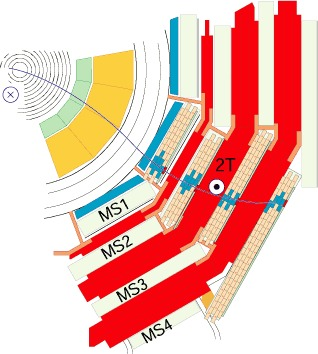
\includegraphics[width=.8\textwidth]{figures/MuStations.jpg}
\caption{The Muon stations in the transverse view}
\label{figs:MuonStation}
\end{figure}
  




\begin{figure}
\centering
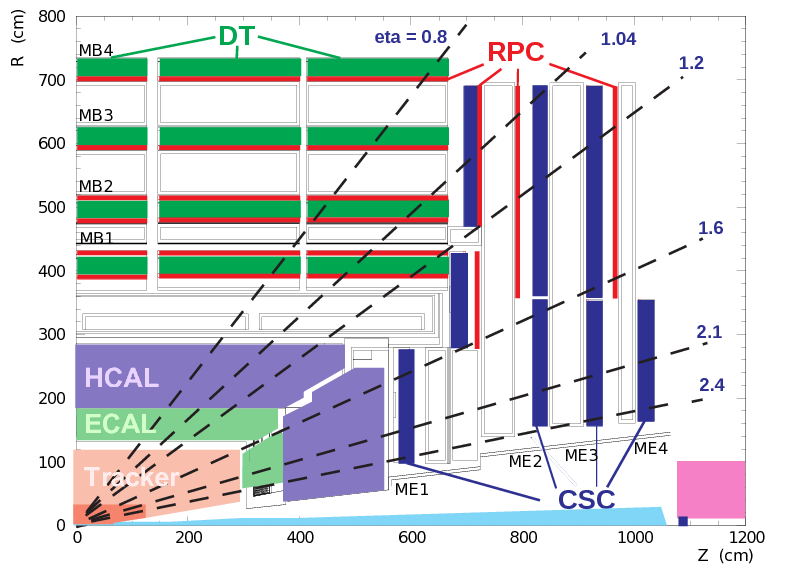
\includegraphics[width=.8\textwidth]{figures/Muonsystem.png}
\caption{Layout of one quarter of the CMS muon system for initial low luminosity running. The 
RPC system is limited to $|\eta| < 1.6$ in the endcap, and for the CSC system only the inner ring of the ME4 chambers  have been deployed. {\color{red} reference the book or the website}}
\label{figs:Muonsystem}
\end{figure}
  


\begin{figure}
\centering
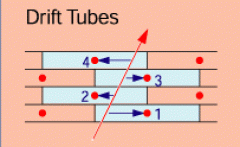
\includegraphics[width=.8\textwidth]{figures/DT.png}
\caption{Layout of the drift tube. }
\label{figs:DT}
\end{figure}

  



 
 
 





